%%%%%%%%%%%%%%
%            %
%   LAYOUT   %
%            %
%%%%%%%%%%%%%%

\documentclass[a4paper,12pt]{article}
\usepackage{geometry}
\geometry{top=2cm, bottom=2cm, left=2.5cm, right=2.5cm}




%%%%%%%%%%%%%%%%
%              %
%   ENCODING   %
%              %
%%%%%%%%%%%%%%%%

\usepackage[T1]{fontenc}    % Use T1 encoding
\usepackage[utf8]{inputenc} % Use UTF-8 encoding for input




%%%%%%%%%%%%%%
%            %
%   IMAGES   %
%            %
%%%%%%%%%%%%%%

\usepackage{graphicx}
% Define a new command for inserting an image
\newcommand{\img}[1]{
    \begin{figure}[h!]
        \centering
        \includegraphics{#1}  % image file path
    \end{figure}
}
\newcommand{\imgw}[2]{
    \begin{figure}[h!]
        \centering
        \includegraphics[width=#2\textwidth]{#1}
    \end{figure}
}
\newcommand{\imgc}[4]{
    \begin{figure}[h!]
        \centering
        \includegraphics[width=#2\textwidth]{#1}
        \caption{#3}  % caption
        \label{#4}  % label
    \end{figure}
}




%%%%%%%%%%%%%%%%
%              %
%   CAPTIONS   %
%              %
%%%%%%%%%%%%%%%%

\usepackage{caption}
\captionsetup[figure]{labelfont=bf}  % Make the figure number bold
\captionsetup[table]{labelfont=bf}




%%%%%%%%%%%%%%%%%%%%%%%%%%%
%                         %
%   SYNTAX HIGHLIGHTING   %
%                         %
%%%%%%%%%%%%%%%%%%%%%%%%%%%

\usepackage{listings}
\usepackage{xcolor}

\definecolor{codegray}{rgb}{0.5,0.5,0.5}
\definecolor{codepurple}{rgb}{0.58,0,0.82}
\definecolor{backcolour}{rgb}{0.95,0.95,0.92}

\lstdefinestyle{csharpstyle}{
    backgroundcolor=\color{backcolour},
    commentstyle=\color{codegray},
    keywordstyle=\color{blue},
    numberstyle=\tiny\color{codegray},
    stringstyle=\color{codepurple},
    basicstyle=\ttfamily\footnotesize,
    breakatwhitespace=false,
    breaklines=true,
    captionpos=b,
    keepspaces=true,
    numbers=left,
    numbersep=5pt,
    showspaces=false,
    showstringspaces=false,
    showtabs=false,
    tabsize=2,
    language=[Sharp]C,
}




%%%%%%%%%%%%%%%%%%%
%                 %
%   TRANSLATION   %
%                 %
%%%%%%%%%%%%%%%%%%%

\usepackage[lithuanian]{babel} % Vertimas tituliniui ir antraštėms




%%%%%%%%%%%%%%%
%             %
%   CONTENT   %
%             %
%%%%%%%%%%%%%%%

\begin{document}

\begin{titlepage}

    \newcommand{\universitetas}{Kauno technologijos universitetas}
    \newcommand{\fakultetas}{Informatikos fakultetas}
    \newcommand{\modulioKodas}{Modulio P170B400}
    \newcommand{\pavadinimas}{„Algoritmų sudarymas ir analizė“}
    \newcommand{\darboTipas}{Laboratorinio darbo ataskaita}
    \newcommand{\laboratorinisDarbas}{Ketvirtas laboratorinis darbas}
    \newcommand{\autorius}{Vardenis Pavardenis IFF-2/2}
    \newcommand{\statusas}{Studentas}
    \newcommand{\destytojasOne}{Asist. Pavardenis Vardenis}
    \newcommand{\destytojasTwo}{doc. Pavardenis Vardenis}
    \newcommand{\destytojai}{Dėstytojai}
    \newcommand{\miestas}{Kaunas}
    \newcommand{\metai}{2024}
    
    \center
    
\includegraphics[width=1.78cm]{nuotraukos/KTU_logo.pdf} \\ [5mm]
    \textbf{\universitetas} \\ [5mm]
    \textbf{\fakultetas} \vfill
    
    \textbf{\modulioKodas} \\ [5mm]
    \LARGE\textbf{\pavadinimas} \\ [10mm]
    \normalsize\textbf{\darboTipas} \\ [5mm]
    \textbf{\laboratorinisDarbas} \vfill
    
    \begin{flushright}
    \rule{0.9\textwidth}{0.4pt} \\ [0.5cm]
    \textbf{\autorius} \\ [5pt]
    \textbf{\statusas} \\ [15pt]
    \textbf{\destytojasOne} \\ [5pt]
    \textbf{\destytojasTwo} \\ [5pt]
    \textbf{\destytojai} \\ [1.5cm]
    \rule{0.9\textwidth}{0.4pt}
    \end{flushright}
    
    \vfill
    \center
    \miestas~\metai
    
    \end{titlepage}

\tableofcontents \newpage

\section{Užduotis}
Parašyti efektyvias rekursinių procedūrų realizacijas, nenaudojant jokių grafinių bibliotekų, kurios generuotų nurodytos struktūros BMP formato paveikslėlį. Šio darbo tikslas yra suprasti ir išanalizuoti rekursinių procedūrų veikimą bei jų efektyvumą.

\textbf{Reikalavimai:}
\begin{enumerate}
    \item \textbf{Realizacijos atvejai:}
    \begin{itemize}
        \item Nurodomas rekursijos gylis.
        \item Generuojamas maksimalaus detalumo paveikslėlis, nurodytiems paveikslėlio matmenims.
    \end{itemize}
    \item \textbf{Programų rezultatas:} Sukurti BMP formato bylas, kurios demonstruotų programos veikimą. (3 balai)
    \item \textbf{Eksperimentinis tyrimas:} Nustatyti darbo laiko ir veiksmų skaičiaus priklausomybę nuo rekursijos gylio arba generuojamo paveikslėlio dydžio (taškų skaičiaus). Gautus rezultatus atvaizduoti grafikais. Grafikus turi sudaryti ne mažiau kaip 5 taškai, o paveikslėlio taškų skaičius turi didėti proporcingai (kartais). (2 balai)
    \item \textbf{Analitinė analizė:} Analitiškai įvertinti procedūrų, kurios generuoja paveikslėlius, veiksmų skaičių ir laiką, sudarant rekurentines lygtis ir jas išsprendžiant. Gautus rezultatus palyginti su eksperimentiniais rezultatais (našumo testais: vykdymo laiku ir veiksmų skaičiumi). (2 balai)
    \item \textbf{Ataskaita:} Paruošti detalią ataskaitą su atliktais skaičiavimais. Ataskaita privalo tenkinti rašto darbų reikalavimus. Visos formulės turi būti rašomos pagal matematikos kanonus. Programų fragmentai neturėtų būti pateikiami tiesiog kaip ekrano kopijos. Rekomenduojama naudoti \LaTeX{} arba Word redaktorius matematinių išraiškų rašymui. (3 balai)
\end{enumerate}

% \begin{figure}[h!]  % 'h!' places image "here" if possible
%     \centering  % Center the image
%     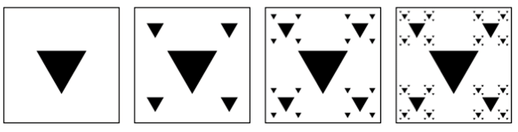
\includegraphics[width=0.8\textwidth]{nuotraukos/Uzduotis.png}
%     \caption{Užduoties siekiamas rezultatas.}
%     \label{fig:problem}
% \end{figure}

\imgc{nuotraukos/Uzduotis.png}{0.8}{Užduoties siekiamas rezultatas.}{}

\section{Kodo fragmentas}

equilateralTriangle bus žymimas $T_eqtriangle(k_x0, ky0, kx1, ky1).$


\lstset{style=csharpstyle}
\begin{lstlisting}
static void equilateralTriangle(byte[] t, (int x, int y) start, (int x, int y) end,
 int pic_height, int l)
{
    int width = Math.Abs(end.x - start.x);
    int height = Math.Abs(end.y - start.y);


    int side = width / 3;// width/3 is the length of the triangle's side
    int triangleHeight = (int)(side * Math.Sqrt(3) / 2);
    int padY = (height / 3 - triangleHeight) / 2;//to fix triangle positioning

    //triangle's vertices
    var v0 = (x: start.x + side, y: start.y + padY + side);
    var v1 = (x: start.x + side * 2, y: start.y + padY + side);
    var v2 = (x: start.x + width / 2, y: start.y + padY + side + triangleHeight);

    triangle(t, v0, v1, v2, pic_height, l);
}

\end{lstlisting}

 

\end{document}
